\documentclass[11pt,A4,french]{article}
\usepackage[lmargin=0.9in,rmargin=0.9in,tmargin=1in,bmargin=1in]{geometry}
\usepackage[utf8]{inputenc}
\usepackage[T1]{fontenc}
\usepackage{amsmath}
\usepackage{amsfonts}
\usepackage{amssymb}
\usepackage[version=4]{mhchem}
\usepackage{stmaryrd}
\usepackage{bbold}
\usepackage{svg}
\usepackage{graphicx}
\usepackage{stfloats}
\usepackage[export]{adjustbox}
\graphicspath{ {./images/} }

\newcommand{\R}{\mathbb{R}}


\title{Projet MOGPL : optimisation équitable }

\author{Zhenyue FU 28620112\\Charles LIN 3812676}
\date{}


\begin{document}
\maketitle
\section*{1) Linéarisation de $f$}

1.1)
$$
\min \sum_{i=1}^{n} a_{i k} z_{i}
$$

$$
\begin{gathered}
\text { s.c. } \sum_{i=1}^{n} a_{i k}=k \\
a_{i k} \in\{0,1\}, i=1, \ldots, n
\end{gathered}
$$

$L_{k}(z)=\sum_{i=1}^{k} z_{(i)}$ représentent les k plus petites composantes de z

Lors de la minimisation de $\sum_{i=1}^{n} a_{i k} z_{i}$ nous mettons les $a_{i k}$ des plus petit $z_{i}$ à 1

Or $sum_{i=1}^{n} a_{i k}=k$ donc on met k $a_{i k}$ à 1

Donc nous récupérons les k $z_{i}$ les plus petits, et donc $L_{k}(z)$


1.2)
$$
\begin{gathered}
\max k r_{k}-\sum_{i=1}^{n} b_{i k} \\
\text { s.c. }
r_{k}-b_{i k} \leq z_{i}(x), i=1, \ldots, n \\
r_k \in \R, b_{i k} \geq 0, i=1, \ldots, n
\end{gathered}
$$

En résolvant 6 programmation linéaires($k=1,\ldots,6$), on obtient:
\begin{align*}
L = (1,3,6,10,17,26)
\end{align*}


1.3)
\begin{equation*} 
\begin{split} 
\sum_{k=1}^{n} w_{k}^{\prime} L_{k}(z(x)) & = \sum_{k=1}^{n-1} (w_k-w_{k+1})L_k + w_nL_n \\
     & = w_1L_1 + \sum_{k=2}^n w_k(L_k-L_{k-1}) \\
     & = w_1z_{1} + \sum_{k=2}^n w_k(z_{k}) \\
     & = \sum_{i=1}^{n} w_{i} z_{(i)}(x) \\
\end{split}
\end{equation*}

\newpage
1.4)
$$
\begin{gathered}
    \max w_1^{\prime}(1 \times r_1 - b_{11} - b_{21}) + w_2^{\prime}(2 \times r_2 - b_{12} - b_{22}) \\
\text { s.c. }\left\{\begin{array}{l}
r_{1}-b_{11} \leq 5 x_{1}+6 x_{2}+4 x_{3}+8 x_{4}+x_{5} \\
r_{1}-b_{21} \leq 3 x_{1}+8 x_{2}+6 x_{3}+2 x_{4}+5 x_{5} \\
r_{2}-b_{12} \leq 5 x_{1}+6 x_{2}+4 x_{3}+8 x_{4}+x_{5} \\
r_{2}-b_{22} \leq 3 x_{1}+8 x_{2}+6 x_{3}+2 x_{4}+5 x_{5} \\
x_{1}+x_{2}+x_{3}+x_{4}+x_{5}=3 \\
\end{array}\right. \\
x_{i} \in\{0,1\}, i=1, \ldots, 5, \indent \text{avec } w_1^{\prime}=1,w_2^{\prime}=1
\end{gathered}
$$

Solution:
\begin{align*}
&z_1 = 18, z_2 = 16\\
&x_1 = 0, x_2 = 1, x_3 = 1, x_4 = 1, x_5=0   
\end{align*}

\section*{2) Application au partage équitable de biens indivisibles}

2.1)

$$
\begin{gathered}
    \max \sum_{k=1}^{n} w_{k}^{\prime}\left(k r_{k}-\sum_{i=1}^{n} b_{i k}\right) \\
    \text { s.c. }\left\{\begin{array}{lr}
    r_{k}-b_{i k} \leq \sum_{j=1}^p u_{ij}x_{ij} \indent i=1, \ldots, n \\
    \sum_{i=1}^n x_{ij} <= 1 \indent \indent \indent j=1, \ldots, p \\
    \end{array}\right. \\
    r_k \in \R, b_{i k} \geq 0, x_{ij} \in\{0,1\},\indent i=1, \ldots, n
\end{gathered}
$$

Avec $w=(3,2,1)$ et $w=(10,3,1)$, on obtient la même solution:
\begin{align*}
& z_1 = 325, z_2 = 335, z_3 = 340 \\
&x_{11} = 1 \\
&x_{23} = 1, x_{25} = 1, x_{26} = 1 \\
&x_{32} = 1, x_{34} = 1 \\
\end{align*}

En maximisant la satisfaction moyenne:
\begin{align*}
&z_1 = 0,
z_2 = 760,
z_3 = 240\\
&x_{21} = 1,x_{22} = 1, x_{23} = 1 \\
&x_{34} = 1,x_{35} = 1, x_{36} = 1 \\
\end{align*}

\newpage
2.2)

\centerline{\includesvg[inkscapelatex=false,width=0.7\columnwidth]{images/22.svg}}
On observe que le temps de résolution à une allure de fonction exponentielle par rapport à n


\section*{3) Application à la selection multicritère de projets}

3.1)
$$
\begin{gathered}
\max \sum_{k=1}^{n} w_{k}^{\prime}\left(k r_{k}-\sum_{i=1}^{n} b_{i k}\right) \\
\text { s.c. }\left\{\begin{array}{l}
r_{k}-b_{i k} \leq = \sum_{j=1}^{p} u_{i j}x_j, i=1, \ldots, n \\
x_i <= 1, i=1, \ldots, n \\
\sum_{i=1}^{p} x_ic_i\leq budget
\end{array}\right. \\
b_{i k} \geq 0, i=1, \ldots, n
\end{gathered}
$$

Avec $w=(2,1)$ et $w=(10,1)$, on obtient la même solution:
\begin{align*}
&z_1 = 21.0, z_2 = 20.0\\
&x_1 = 1.0, x_2 = 0.0, x_3 = 0.0, x_4 = 1.0\\
\end{align*}

En maximisant la satisfaction moyenne:
\begin{align*}
&z_1 = 36.0, z_2 = 6.0\\
&x_1 = 1.0, x_2 = 0.0, x_3 = 1.0, x_4 = 0.0 \\
\end{align*}

\newpage

3.2)
\begin{figure}[h!]
    \centering
    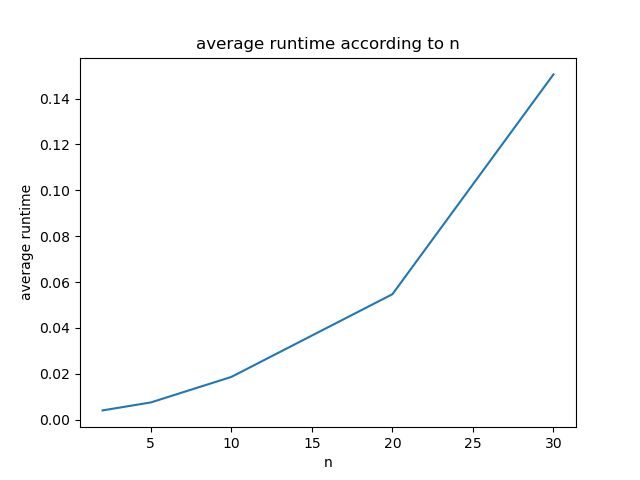
\includegraphics[max width=0.45\textwidth]{images/32_n.png}
    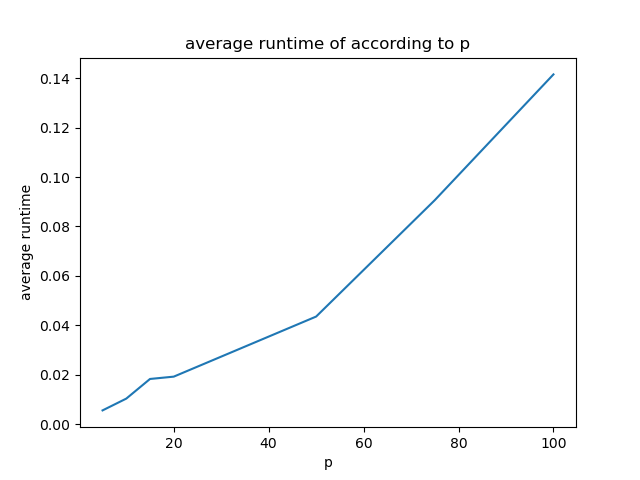
\includegraphics[max width=0.45\textwidth]{images/32_p.png}
\end{figure}

On observe que le temps de résolution du programme est beaucoup plus impacter par n que par p, elle a une allure exponentielle par rapport à n, et une allure affine par rapport à p.

\section*{4) Application à la recherche d'un chemin robuste dans un graphe}

4.1) 

for $G=(V,E)$ 
$$
\begin{gathered}
\min \sum_{i,j\in V} t_{ij}x_{ij} \\
\text { s.c. }
\sum_{vj \in E} x_{vj} - \sum_{jv \in E} x_{jv} = c_v , \forall v \in V \\
x_{i j} \in {0,1}, \forall i,j \in E \\
\text{où } c_v = \begin{cases}
    1 &\text{if } v=a\\
    -1 &\text{if } v=g\\
    0 &\text{else}\\
\end{cases}
\end{gathered}
$$
On a résolu le Programmation Linaire avec les résultats suivants dans Figure 1:

\begin{figure}[ht!]
    \centering
    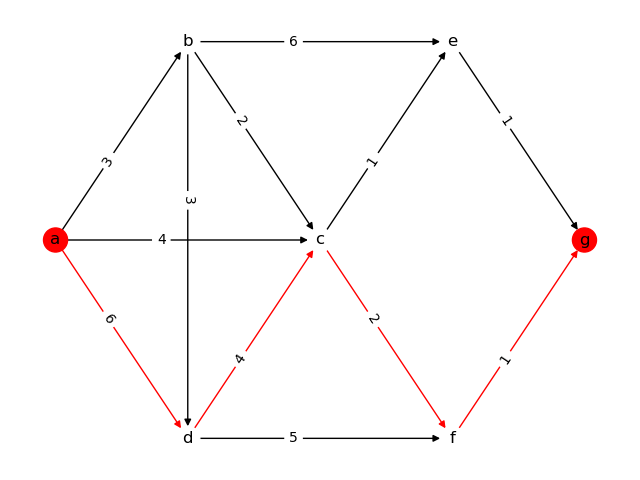
\includegraphics[max width=0.45\textwidth]{images/shortest_path_4_1_s1.png}
    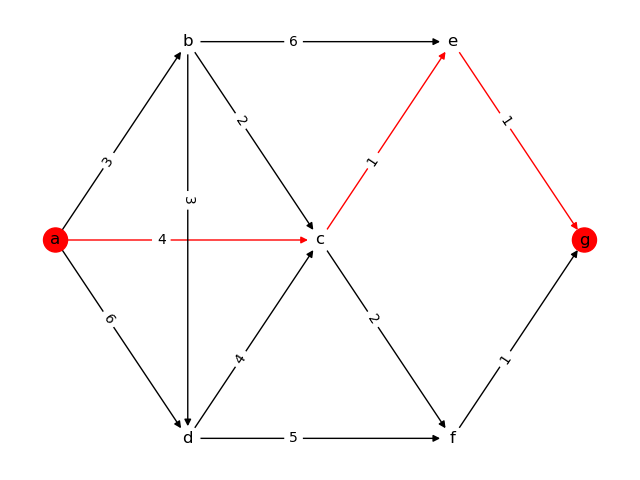
\includegraphics[max width=0.45\textwidth]{images/shortest_path_4_1_s2.png}
    \caption{Shortest path with s1 and s2}
    \label{fig:my_label}
\end{figure}


4.2)
$$
\begin{gathered}
    \max \sum_{k=1}^{n} w_{k}^{\prime}\left(k r_{k}-\sum_{i=1}^{n} b_{i k}\right) \\
    \text { s.c. }\left\{\begin{array}{lr}
    r_{k}-b_{i k} + \sum_{u,v\in V} t_{uv}^ix_{uv} \leq 0 \indent i=1, \ldots, n \\
    \sum_{vj \in E} x_{vj} - \sum_{jv \in E} x_{jv} = c_v , \forall v \in V \\
    \end{array}\right. \\
    r_k \in \R, b_{i k} \geq 0, i=1, \ldots, n,\indent x_{ij} \in \{0,1\} \indent \forall i,j \in E \\
    \text{où } c_v = \begin{cases}
    1 &\text{if } v=a\\
    -1 &\text{if } v=g\\
    0 &\text{else}\\
\end{cases}
\end{gathered}
$$

On a résolu le Programmation Linaire avec les résultats suivants dans Figure 2.

\begin{figure}[ht!]
    \centering
    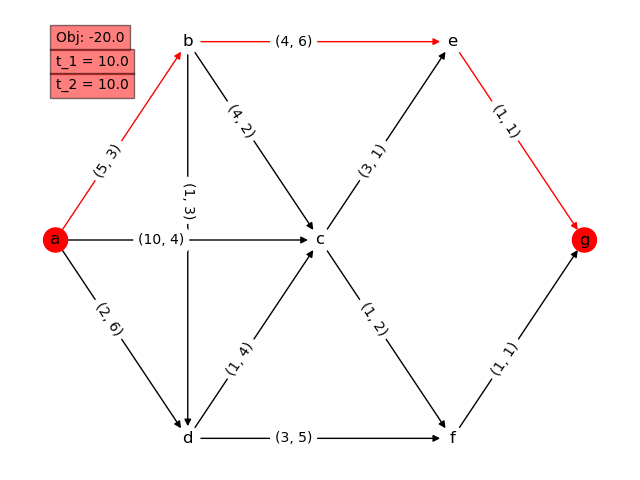
\includegraphics[max width=0.45\textwidth]{images/path_4_2.png}
    \caption{Path 4.2}
    \label{fig:my_label}
\end{figure}

\par
4.3) 
Pour chaque alpha, nous obtenons exactement le même chemin, w n'a donc pas d'incidence sur la solution.
Tous les chemins pour chaque itération et chaque alpha sont stockés dans le fichier 4\_3.

\end{document}